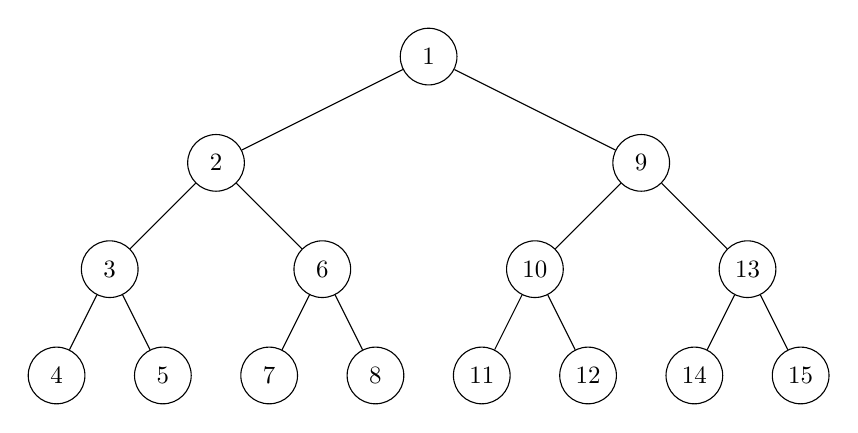
\begin{tikzpicture}[nodeStyle/.style={circle, draw, minimum size=0.8cm}, scale=0.9, transform shape]
    % Root
    \node[nodeStyle] (1) at (0, 0) {1};

    % Layer 1
    \node[nodeStyle] (2) at (-3, -1.5) {2};
    \node[nodeStyle] (9) at ( 3, -1.5) {9};

    % Layer 2
    \node[nodeStyle]  (3) at (-4.5, -3)  {3};
    \node[nodeStyle]  (6) at (-1.5, -3)  {6};
    \node[nodeStyle] (10) at ( 1.5, -3) {10};
    \node[nodeStyle] (13) at ( 4.5, -3) {13};

    % Layer 3
    \node[nodeStyle]  (4) at (-5.25, -4.5)  {4};
    \node[nodeStyle]  (5) at (-3.75, -4.5)  {5};
    \node[nodeStyle]  (7) at (-2.25, -4.5)  {7};
    \node[nodeStyle]  (8) at (-0.75, -4.5)  {8};
    \node[nodeStyle] (11) at ( 0.75, -4.5) {11};
    \node[nodeStyle] (12) at ( 2.25, -4.5) {12};
    \node[nodeStyle] (14) at ( 3.75, -4.5) {14};
    \node[nodeStyle] (15) at ( 5.25, -4.5) {15};


    % Edges
    \draw (1) -- (2);
    \draw (1) -- (9);

    \draw (2) -- (3);
    \draw (2) -- (6);
    \draw (9) -- (10);
    \draw (9) -- (13);

    \draw (3) -- (4);
    \draw (3) -- (5);
    \draw (6) -- (7);
    \draw (6) -- (8);
    \draw (10) -- (11);
    \draw (10) -- (12);
    \draw (13) -- (14);
    \draw (13) -- (15);
\end{tikzpicture}